% Three transition slides: the river network as an electrical circuit.
% To use in the main deck: copy the three frames below, the figures/ folder,
% and the packages marked "needed by the frames" into the main preamble.
\documentclass[aspectratio=169]{beamer}

% needed by the frames
\usepackage{amsmath}
\usepackage{booktabs}
\usepackage{tikz}
\usepackage[european]{circuitikz}
\usetikzlibrary{decorations.pathreplacing,arrows.meta}
\graphicspath{{figures/}}

\setbeamertemplate{navigation symbols}{}

\begin{document}

% ---------------------------------------------------------------- slide 1
\begin{frame}{From river geometry to an electrical network}
\begin{columns}[T,onlytextwidth]
\begin{column}{0.40\textwidth}
\centering
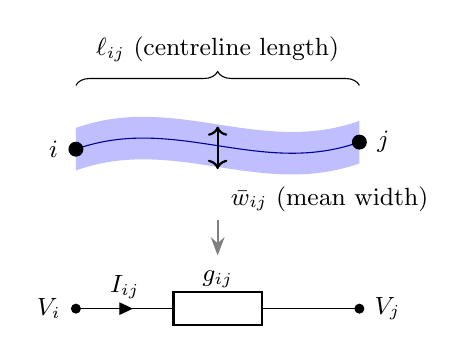
\begin{tikzpicture}[scale=0.9, every node/.style={font=\small}]
  % the channel as a band between two junctions
  \fill[blue!25] (0,2.55) .. controls (1.4,3.05) and (2.6,2.15) .. (4,2.65)
                 -- (4,2.05) .. controls (2.6,1.55) and (1.4,2.45) .. (0,1.95) -- cycle;
  \draw[blue!60!black] (0,2.25) .. controls (1.4,2.75) and (2.6,1.85) .. (4,2.35);
  \fill[black] (0,2.25) circle (3pt) node[left=3pt] {$i$};
  \fill[black] (4,2.35) circle (3pt) node[right=3pt] {$j$};
  \draw[<->, thick] (2.0,1.97) -- (2.0,2.57);
  \node[right] at (2.05,1.55) {$\bar w_{ij}$ (mean width)};
  \draw[decorate, decoration={brace, amplitude=5pt}] (0,3.15) -- (4,3.15)
       node[midway, above=5pt] {$\ell_{ij}$ (centreline length)};
  % mapping arrow
  \draw[-{Stealth}, thick, gray] (2,1.25) -- (2,0.75);
  % the same channel as a resistor
  \draw (0,0) node[circ]{} node[left=2pt] {$V_i$}
        to[R, l=$g_{ij}$, i>^=$I_{ij}$] (4,0) node[circ]{} node[right=2pt] {$V_j$};
\end{tikzpicture}

\vspace{2mm}
{\footnotesize Each channel becomes a resistor between its two junctions.}
\end{column}

\begin{column}{0.56\textwidth}
\begin{block}{1. Geometric weighting}
\small
\[ g_{ij} = \frac{\bar w_{ij}}{\ell_{ij}} \qquad \Big(\text{like } G \propto \tfrac{A}{L}\Big) \]
Width/length acts as channel conductance (depth taken as constant). Weights are normalised.
\end{block}

\begin{block}{2. Electrical network}
\small
\begin{itemize}\setlength{\itemsep}{0pt}
  \item Junctions are nodes and channels are resistors.
  \item Inlets are held at $V=1$ and outlets at $V=0$.
  \item Ohm's law on each edge: $I_{ij} = g_{ij}\,(V_i - V_j)$
  \item Kirchhoff at every internal node: $\sum_j I_{ij} = 0$
\end{itemize}
\vspace{2mm}
\centerline{$L\,V = I_{\text{ext}}, \qquad L_{ii} = \textstyle\sum_j g_{ij}, \quad L_{ij} = -g_{ij}$}
\vspace{2mm}
Solving for $V$ gives the current on every channel.
\end{block}
\end{column}
\end{columns}
\end{frame}

% ---------------------------------------------------------------- slide 2
\begin{frame}{Evolution of network conductance}
\begin{columns}[T,onlytextwidth]
\begin{column}{0.49\textwidth}
\centering
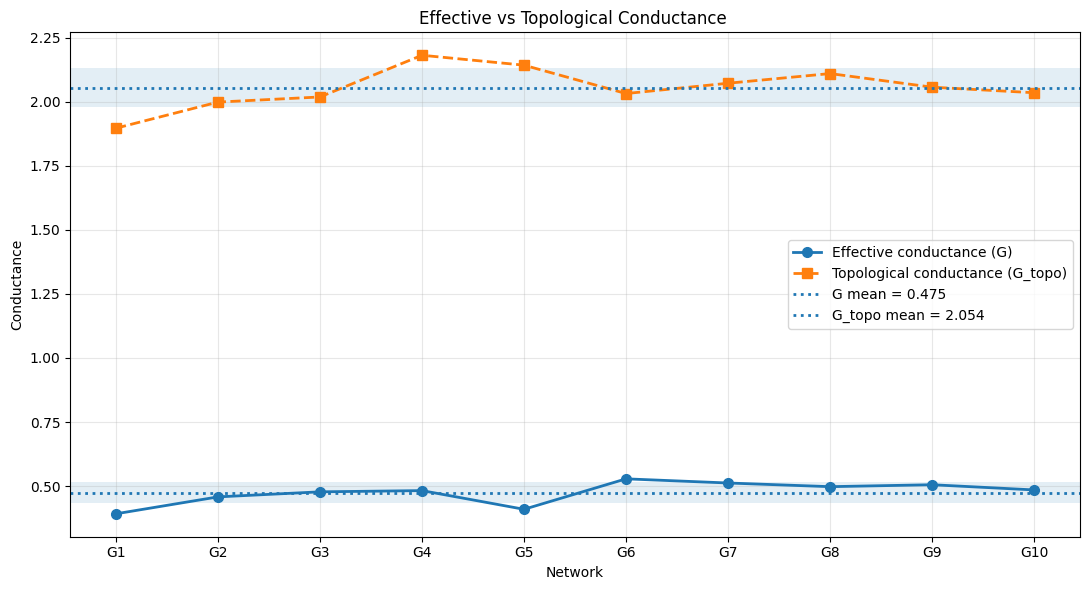
\includegraphics[width=\linewidth]{G_vs_Gtopo.png}

\vspace{1mm}
\scriptsize
\begin{itemize}\setlength{\itemsep}{1pt}
  \item $G_{\text{topo}}$: every channel has unit conductance, so it only changes with connectivity (nodes, edges, inlet and outlet sets). It stays within about 1.90--2.18.
  \item $G$: geometrically weighted, so it reflects changes in both topology and geometry.
  \item The two are on different scales and cannot be compared directly.
\end{itemize}
\end{column}

\begin{column}{0.49\textwidth}
\centering
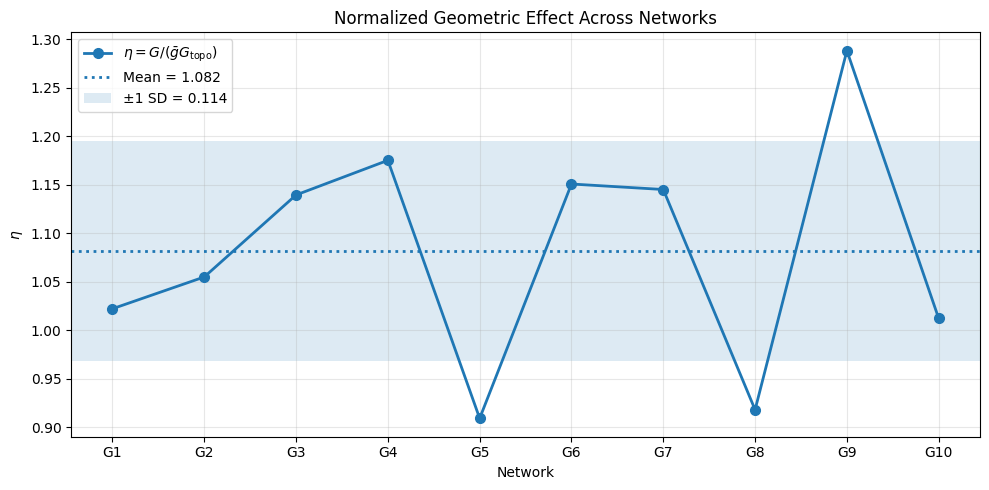
\includegraphics[width=\linewidth]{eta.png}

\vspace{1mm}
\scriptsize
Normalised geometric effect: \;$\eta = \dfrac{G}{\bar g\, G_{\text{topo}}}$

\vspace{1mm}
\begin{tabular}{@{}lp{0.78\linewidth}@{}}
\toprule
$\eta = 1$ & same conductance as uniform weights \\
$\eta < 1$ & width and length arrangement hinders flow \\
$\eta > 1$ & width and length arrangement favours flow \\
\bottomrule
\end{tabular}
\end{column}
\end{columns}

\vspace{2mm}
\begin{center}
\small\alert{$\eta$ fluctuates (0.91--1.29) instead of following a trend. Why?}
\end{center}
\end{frame}

% ---------------------------------------------------------------- slide 3
\begin{frame}{Why $\eta$ changes: edge conductances or pathways?}
\centering
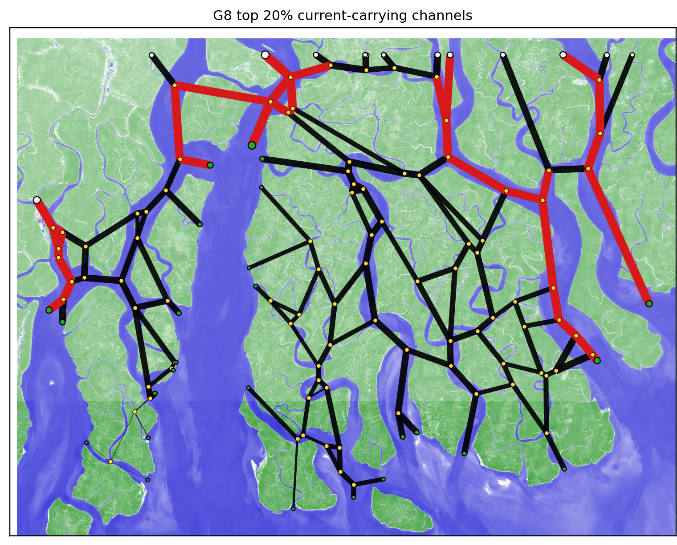
\includegraphics[height=4.75cm]{G8_current.png}\hfill
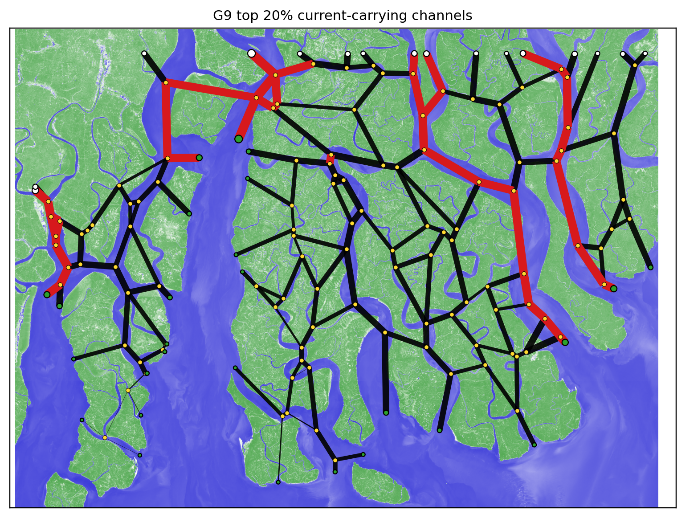
\includegraphics[height=4.75cm]{G9_current.png}

\vspace{1.5mm}
\begin{columns}[c,onlytextwidth]
\begin{column}{0.33\textwidth}
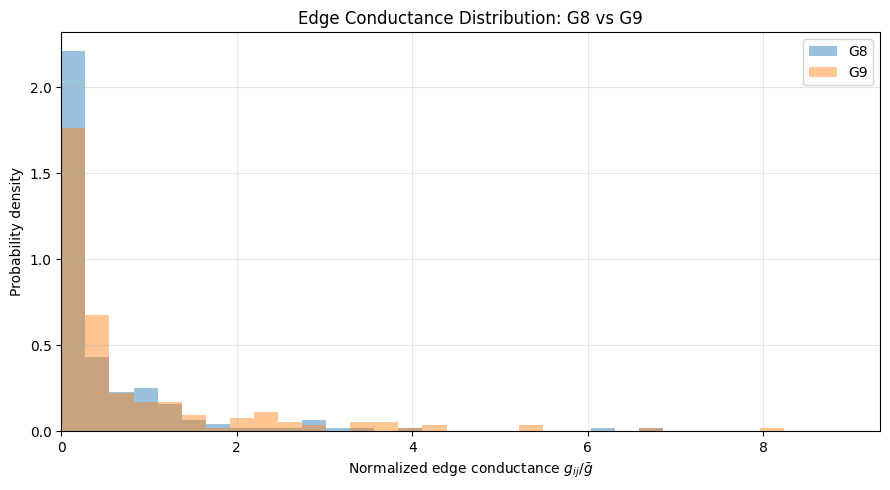
\includegraphics[height=2.45cm]{edge_conductance_hist.png}
\end{column}
\begin{column}{0.65\textwidth}
\small
\begin{itemize}\setlength{\itemsep}{2pt}
  \item Edge conductance distributions are nearly the same.
  \item The main current paths (red) are similar.
  \item G9 adds parallel low-conductance routes: $\eta$ rises from 0.92 to 1.29.
\end{itemize}
\end{column}
\end{columns}
\end{frame}

\end{document}
